\documentclass[10pt]{article}

\usepackage{parskip}
\usepackage[margin=1in]{geometry} 
\usepackage{tikz}
\usetikzlibrary{positioning}
\usepackage{amsmath,amsthm,amssymb, graphicx, multicol, array}
\usepackage{enumitem}
\usepackage{amssymb}
\usepackage{float}
\usepackage{href-ul}
 
\newcommand{\N}{\mathbb{N}}
\newcommand{\Z}{\mathbb{Z}}
 
\newenvironment{problem}[2][Problem]{\begin{trivlist}
\item[\hskip \labelsep {\bfseries #1}\hskip \labelsep {\bfseries #2.}]}{\end{trivlist}}

\begin{document}
 
\title{Foundations of causal inference (cont.)}
\author{Jakob Sverre Alexandersen\\
GRA4158 Marketing and the Analysis of Experiments and Quasi-Experiments\\
Lecture 4}
\maketitle

\tableofcontents
\newpage
\section{Good vs. bad controls}
\subsection{Bad controls}
\begin{itemize}
    \item We talked about that including covariates as controls can be a good strategy to \textbf{reduce error variance and bias (selection bias)} in the focal estimate 
    \item However, that can be harmful if we include the wrong control variables
\end{itemize}
\subsection{Causal diagrams --- Directed Acyclical Graphs (DAG)}
\begin{itemize}
    \item DAGs are often used to represent causal path diagrams 
    \item Consist of nodes that represent variables, and vertices that depict direct causal effects 
    \item A simple DAG:
    \begin{center}
        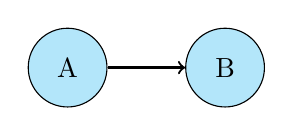
\begin{tikzpicture}[
            node/.style={circle, draw, minimum size=1cm, fill=cyan!30}
        ]
            \node[node] (A) at (0, 0) {A};
            \node[node] (B) at (2, 0) {B};
            \draw[->, thick] (A) -- (B);
        \end{tikzpicture}
    \end{center}
    \item DAGs help to understand the causal order of variables, which is important for correct causal inference
\end{itemize}
\subsubsection{Some important concepts in DAGs}
\begin{itemize}
    \item A causal path is a sequence of nodes where we follow the arrows of the graph: 
    \item All other paths are non-causal, and may induce ``spurious'' associations between X and Y
    \begin{itemize}
        \item Basically, any path from X to Y where we also go against the direction of an arrow
    \end{itemize}
\end{itemize}

\textbf{Some examples:}
\begin{center}
    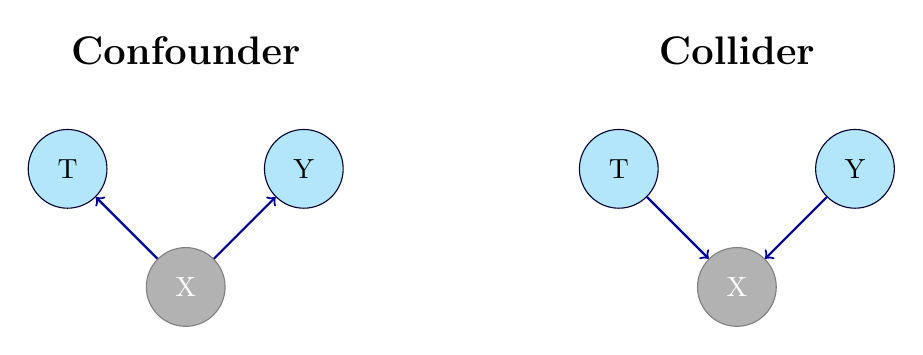
\begin{tikzpicture}[
        darkblue/.style={circle, draw=blue!20!black, fill=cyan!30, text=black, minimum size=1cm},
        gray/.style={circle, draw=gray, fill=gray!60, text=white, minimum size=1cm},
        node distance=2.5cm
    ]
    
    % Confounder diagram
    \node[font=\Large\bfseries] at (0, 2.5) {Confounder};
    \node[darkblue] (T1) at (-1.5, 1) {T};
    \node[darkblue] (Y1) at (1.5, 1) {Y};
    \node[gray] (X1) at (0, -0.5) {X};
    \draw[->, thick, blue!60!black] (X1) -- (T1);
    \draw[->, thick, blue!60!black] (X1) -- (Y1);
    
    % Collider diagram
    \node[font=\Large\bfseries] at (7, 2.5) {Collider};
    \node[darkblue] (T2) at (5.5, 1) {T};
    \node[darkblue] (Y2) at (8.5, 1) {Y};
    \node[gray] (X2) at (7, -0.5) {X};
    \draw[->, thick, blue!60!black] (T2) -- (X2);
    \draw[->, thick, blue!60!black] (Y2) -- (X2);
    
    \end{tikzpicture}
\end{center}
\begin{itemize}
    \item In both cases, T has no causal path to Y, but spurious paths through X
    \item Incorrectly utilizing X can represent a potential threat to causal inference
\end{itemize}
\textbf{Confounder are good controls}
\begin{itemize}
    \item We need to include X into the analysis to avoid bias in the estimation
    \item Confounding can be more complex than the simple model that we used before:
\end{itemize}
\begin{center}
    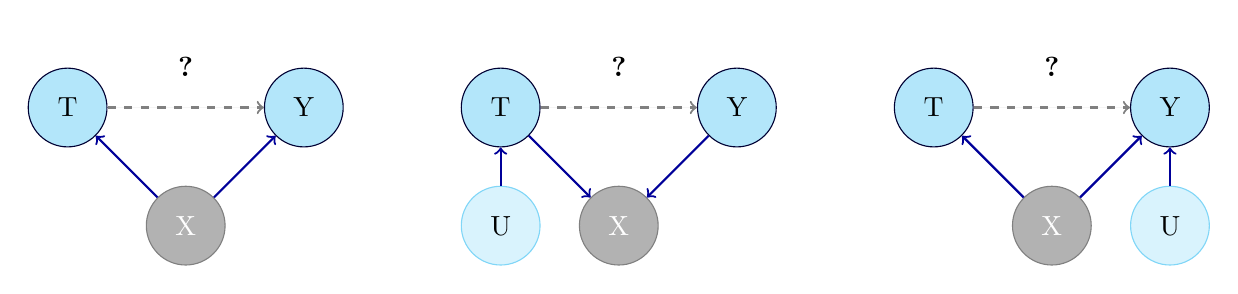
\begin{tikzpicture}[
        darkblue/.style={circle, draw=blue!20!black, fill=cyan!30, text=black, minimum size=1cm},
        gray/.style={circle, draw=gray, fill=gray!60, text=white, minimum size=1cm},
        lightblue/.style={circle, draw=cyan!50, fill=cyan!15, text=black, minimum size=1cm},
        node distance=2.5cm
    ]
    
    % Left diagram - Confounder
    \node[darkblue] (T1) at (0, 1) {T};
    \node[darkblue] (Y1) at (3, 1) {Y};
    \node[gray] (X1) at (1.5, -0.5) {X};
    \draw[->, thick, blue!60!black] (X1) -- (T1);
    \draw[->, thick, blue!60!black] (X1) -- (Y1);
    \draw[->, thick, dashed, gray] (T1) -- node[above, font=\bfseries, text=black] {?} (Y1);
    
    % Middle diagram - Mediator with confounder
    \node[darkblue] (T2) at (5.5, 1) {T};
    \node[darkblue] (Y2) at (8.5, 1) {Y};
    \node[gray] (X2) at (7, -0.5) {X};
    \node[lightblue] (U2) at (5.5, -0.5) {U};
    \draw[->, thick, blue!60!black] (U2) -- (T2);
    \draw[->, thick, blue!60!black] (T2) -- (X2);
    \draw[->, thick, blue!60!black] (Y2) -- (X2);
    \draw[->, thick, dashed, gray] (T2) -- node[above, font=\bfseries, text=black] {?} (Y2);
    
    % Right diagram - Confounder with unmeasured variable
    \node[darkblue] (T3) at (11, 1) {T};
    \node[darkblue] (Y3) at (14, 1) {Y};
    \node[gray] (X3) at (12.5, -0.5) {X};
    \node[lightblue] (U3) at (14, -0.5) {U};
    \draw[->, thick, blue!60!black] (X3) -- (T3);
    \draw[->, thick, blue!60!black] (X3) -- (Y3);
    \draw[->, thick, blue!60!black] (U3) -- (Y3);
    \draw[->, thick, dashed, gray] (T3) -- node[above, font=\bfseries, text=black] {?} (Y3);
    
    \end{tikzpicture}
\end{center}
\newpage 
\textbf{Collider are bad controls}
\begin{itemize}
    \item In its simple form, a collider is a common outcome to both W and Y
    \item Controlling for X will bias the W-Y relationship 
    \begin{itemize}
        \item We sbould NOT include X in the regression $\to $ it is a bad control 
    \end{itemize}
\end{itemize}
\begin{center}
    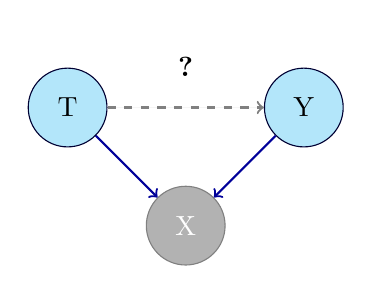
\begin{tikzpicture}[
        darkblue/.style={circle, draw=blue!20!black, fill=cyan!30, text=black, minimum size=1cm},
        gray/.style={circle, draw=gray, fill=gray!60, text=white, minimum size=1cm},
        lightblue/.style={circle, draw=cyan!50, fill=cyan!15, text=black, minimum size=1cm},
        node distance=2.5cm
    ]
    
    % Left diagram - Confounder
    \node[darkblue] (T1) at (0, 1) {T};
    \node[darkblue] (Y1) at (3, 1) {Y};
    \node[gray] (X1) at (1.5, -0.5) {X};
    \draw[->, thick, blue!60!black] (T1) -- (X1);
    \draw[->, thick, blue!60!black] (Y1) -- (X1);
    \draw[->, thick, dashed, gray] (T1) -- node[above, font=\bfseries, text=black] {?} (Y1);
    \end{tikzpicture}
\end{center}

\textbf{Why are colliders bad controls?}
\begin{itemize}
    \item Assume in the population talent and attractiveness of a celebrity are completely unrelated and they both affect success
\end{itemize}
\begin{center}
    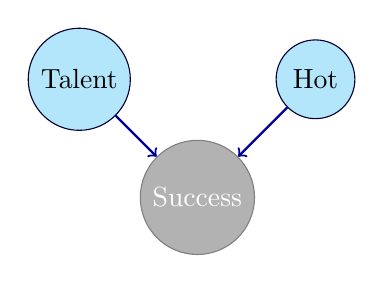
\begin{tikzpicture}[
        darkblue/.style={circle, draw=blue!20!black, fill=cyan!30, text=black, minimum size=1cm},
        gray/.style={circle, draw=gray, fill=gray!60, text=white, minimum size=1cm},
        lightblue/.style={circle, draw=cyan!50, fill=cyan!15, text=black, minimum size=1cm},
        node distance=2.5cm
    ]
    
    % Left diagram - Confounder
    \node[darkblue] (T1) at (0, 1) {Talent};
    \node[darkblue] (Y1) at (3, 1) {Hot};
    \node[gray] (X1) at (1.5, -0.5) {Success};
    \draw[->, thick, blue!60!black] (T1) -- (X1);
    \draw[->, thick, blue!60!black] (Y1) -- (X1);
    % \draw[->, thick, dashed, gray] (T1) -- node[above, font=\bfseries, text=black] {?} (Y1);
    \end{tikzpicture}
\end{center}

\begin{itemize}
    \item Success is a collider (common outcome) for the relationship between talent and attractiveness
    \begin{center}
        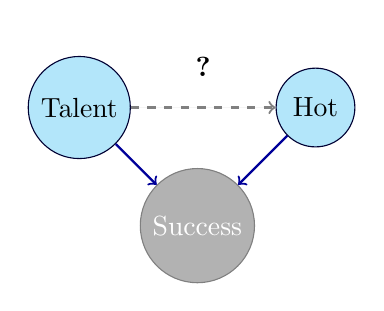
\begin{tikzpicture}[
            darkblue/.style={circle, draw=blue!20!black, fill=cyan!30, text=black, minimum size=1cm},
            gray/.style={circle, draw=gray, fill=gray!60, text=white, minimum size=1cm},
            lightblue/.style={circle, draw=cyan!50, fill=cyan!15, text=black, minimum size=1cm},
            node distance=2.5cm
        ]
        
        % Left diagram - Confounder
        \node[darkblue] (T1) at (0, 1) {Talent};
        \node[darkblue] (Y1) at (3, 1) {Hot};
        \node[gray] (X1) at (1.5, -0.5) {Success};
        \draw[->, thick, blue!60!black] (T1) -- (X1);
        \draw[->, thick, blue!60!black] (Y1) -- (X1);
        \draw[->, thick, dashed, gray] (T1) -- node[above, font=\bfseries, text=black] {?} (Y1);
        \end{tikzpicture}
    \end{center}
    \item Controlling for success will bias our estimated relationship between talent and attractiveness
\end{itemize}
\textbf{The reason}
\begin{itemize}
    \item If you see a successful celebrity who is \textbf{not attractive}, they must be \textbf{highly talented}
    \item If you see a successful celebrity who is \textbf{not talented}, they must be \textbf{highly attractive}
    \item For any given level of success (controlling for success)
    \begin{itemize}
        \item Having high talent will typically coincide with lower levels of attractiveness
        \item Having low talent will typically coincide with higher levels of attractiveness
        \item \textbf{Negative relationship}
    \end{itemize}
\end{itemize}
\newpage 
\subsection{A marketing example}
\begin{itemize}
    \item Do creative ads have an effect on buying intention of customers?
    \begin{itemize}
        \item Let's assume that ad creativity is randomized (i.e., has no relation with buying intention)
        \item Creative ads only affect whether people click (it does not change their buying intention)
        \item Buying intention also affects whether people click 
        \begin{center}
            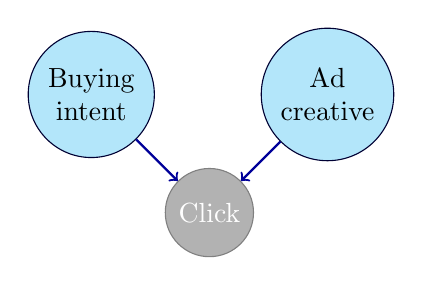
\begin{tikzpicture}[
                darkblue/.style={circle, draw=blue!20!black, fill=cyan!30, text=black, minimum size=1cm},
                gray/.style={circle, draw=gray, fill=gray!60, text=white, minimum size=1cm},
                lightblue/.style={circle, draw=cyan!50, fill=cyan!15, text=black, minimum size=1cm},
                node distance=2.5cm
            ]
            
            % Left diagram - Confounder
            \node[darkblue, align=center] (T1) at (0, 1) {Buying\\intent};
            \node[darkblue, align=center] (Y1) at (3, 1) {Ad\\creative};
            \node[gray] (X1) at (1.5, -0.5) {Click};
            \draw[->, thick, blue!60!black] (T1) -- (X1);
            \draw[->, thick, blue!60!black] (Y1) -- (X1);
            % \draw[->, thick, dashed, gray] (T1) -- node[above, font=\bfseries, text=black] {?} (Y1);
            \end{tikzpicture}
        \end{center}
        \item Controlling for click will bias an estimated relationship between ad creative and intent $\to $ \textbf{collider bias}
    \end{itemize}
    \item If people who click have low intent, then they saw the creative ad 
    \item If people who click saw the non-creative ad, then they might have high intent 
    \item \textbf{Conditional on click} there is a \textbf{negative} relationship between intent and creativity
    \item If we run a regression with $\text{Intent} = \alpha + \beta\text{ Creative} + \gamma\text{ Click} + \epsilon $
    \begin{itemize}
        \item We will find that $\beta $ is negative 
        \item It is biased because the population effect is zero
    \end{itemize}
    \item However, when we run $\text{Intent} = \alpha + \beta\text{ Creative} + \zeta $
    \begin{itemize}
        \item We will find that $\beta $ is close to zero (insignificant)
    \end{itemize}
\end{itemize}
\subsection{Some more examples --- another collider}
\begin{center}
    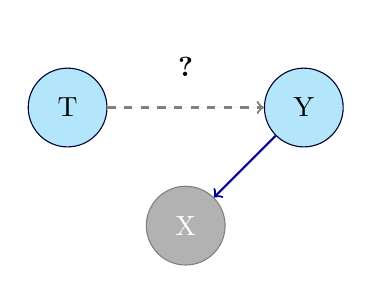
\begin{tikzpicture}[
        darkblue/.style={circle, draw=blue!20!black, fill=cyan!30, text=black, minimum size=1cm},
        gray/.style={circle, draw=gray, fill=gray!60, text=white, minimum size=1cm},
        lightblue/.style={circle, draw=cyan!50, fill=cyan!15, text=black, minimum size=1cm},
        node distance=2.5cm
    ]
    
    % Left diagram - Confounder
    \node[darkblue] (T1) at (0, 1) {T};
    \node[darkblue] (Y1) at (3, 1) {Y};
    \node[gray] (X1) at (1.5, -0.5) {X};
    % \draw[->, thick, blue!60!black] (T1) -- (X1);
    \draw[->, thick, blue!60!black] (Y1) -- (X1);
    \draw[->, thick, dashed, gray] (T1) -- node[above, font=\bfseries, text=black] {?} (Y1);
    \end{tikzpicture}
\end{center}
\begin{itemize}
    \item Same problem, but X is not directly affected by T, but only indirectly through Y
    \item Including X in the regression will similiarly bias the effect of T on Y (only if T has an effect)
    \begin{itemize}
        \item Any outcome of Y is a bad control
    \end{itemize}
\end{itemize}
\newpage 
\subsection{Some more examples ---  mediator as control?}
\begin{center}
    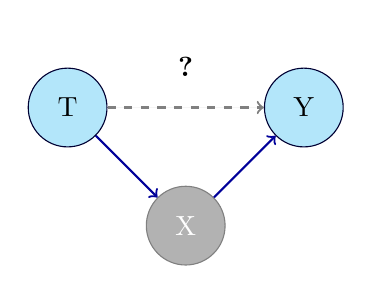
\begin{tikzpicture}[
        darkblue/.style={circle, draw=blue!20!black, fill=cyan!30, text=black, minimum size=1cm},
        gray/.style={circle, draw=gray, fill=gray!60, text=white, minimum size=1cm},
        lightblue/.style={circle, draw=cyan!50, fill=cyan!15, text=black, minimum size=1cm},
        node distance=2.5cm
    ]
    
    % Left diagram - Confounder
    \node[darkblue] (T1) at (0, 1) {T};
    \node[darkblue] (Y1) at (3, 1) {Y};
    \node[gray] (X1) at (1.5, -0.5) {X};
    \draw[->, thick, blue!60!black] (T1) -- (X1);
    \draw[->, thick, blue!60!black] (X1) -- (Y1);
    \draw[->, thick, dashed, gray] (T1) -- node[above, font=\bfseries, text=black] {?} (Y1);
    \end{tikzpicture}
\end{center}
\begin{itemize}
    \item X is an outcome of T and it affects Y $\to $ it is a mediatior
    \item Adding X as a control changes the interpretation of the effect 
    \begin{itemize}
        \item We do not estimate the total effect (average treatment effect) anymore
        \item We estimate a form of direct effect (conditional on X being equal)
    \end{itemize}
\end{itemize}
\begin{center}
    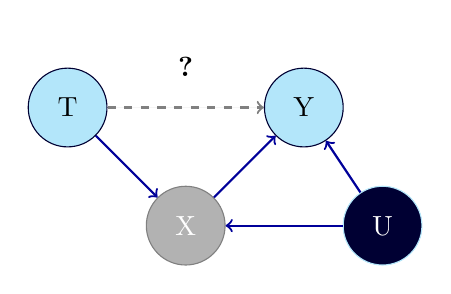
\begin{tikzpicture}[
        darkblue/.style={circle, draw=blue!20!black, fill=cyan!30, text=black, minimum size=1cm},
        blue/.style={circle, draw=cyan!30, fill=blue!20!black, text=white, minimum size=1cm},
        gray/.style={circle, draw=gray, fill=gray!60, text=white, minimum size=1cm},
        lightblue/.style={circle, draw=cyan!50, fill=cyan!15, text=black, minimum size=1cm},
        node distance=2.5cm
    ]
    
    % Left diagram - Confounder
    \node[darkblue] (T1) at (0, 1) {T};
    \node[darkblue] (Y1) at (3, 1) {Y};
    \node[blue] (u) at (4, -0.5) {U};
    \node[gray] (X1) at (1.5, -0.5) {X};
    \draw[->, thick, blue!60!black] (T1) -- (X1);
    \draw[->, thick, blue!60!black] (u) -- (X1);
    \draw[->, thick, blue!60!black] (u) -- (Y1);
    \draw[->, thick, blue!60!black] (X1) -- (Y1);
    \draw[->, thick, dashed, gray] (T1) -- node[above, font=\bfseries, text=black] {?} (Y1);
    \end{tikzpicture}
\end{center}
\begin{itemize}
    \item Mediator as a control is dangerous if there are unobserved confounders on the X-Y relationship
    \begin{itemize}
        \item The total effect is unbiased (i.e., when ignoring X)
        \item The direct effect is biased (i.e., when including X as a control without including U)
    \end{itemize}
\end{itemize}
\subsection{A more complex marketing example}
\begin{itemize}
    \item Let's add \textbf{conversion/purchases}
    \begin{itemize}
        \item Similar like before; ad creativity is randomized and only affects clicks not intent; and bying intention affects clicks 
        \item \textbf{Only buying intention} affects purchase, but only people who click can also purchase 
        \item \textbf{Buying intention is unobserved }
    \end{itemize}
\end{itemize}
\begin{center}
    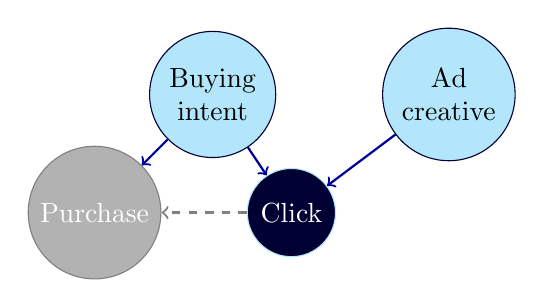
\begin{tikzpicture}[
        darkblue/.style={circle, draw=blue!20!black, fill=cyan!30, text=black, minimum size=1cm},
        blue/.style={circle, draw=cyan!30, fill=blue!20!black, text=white, minimum size=1cm},
        gray/.style={circle, draw=gray, fill=gray!60, text=white, minimum size=1cm},
        lightblue/.style={circle, draw=cyan!50, fill=cyan!15, text=black, minimum size=1cm},
        node distance=2.5cm
    ]
    
    % Left diagram - Confounder
    \node[darkblue, align=center] (T1) at (1.5, 1) {Buying\\intent};
    \node[darkblue, align=center] (Y1) at (4.5, 1) {Ad\\creative};
    \node[blue] (u) at (2.5, -0.5) {Click};
    \node[gray] (X1) at (0, -0.5) {Purchase};
    \draw[->, thick, blue!60!black] (T1) -- (X1);
    \draw[->, thick, blue!60!black] (T1) -- (u);
    \draw[->, thick, gray, dashed] (u) -- (X1);
    \draw[->, thick, blue!60!black] (Y1) -- (u);
    % \draw[->, thick, blue!60!black] (X1) -- (Y1);
    % \draw[->, thick, dashed, gray] (T1) -- node[above, font=\bfseries, text=black] {?} (Y1);
    \end{tikzpicture}
\end{center}
\newpage 
\subsection{Some more examples --- neutral or bad control?}
\begin{center}
    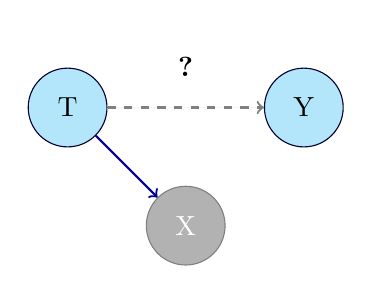
\begin{tikzpicture}[
        darkblue/.style={circle, draw=blue!20!black, fill=cyan!30, text=black, minimum size=1cm},
        gray/.style={circle, draw=gray, fill=gray!60, text=white, minimum size=1cm},
        lightblue/.style={circle, draw=cyan!50, fill=cyan!15, text=black, minimum size=1cm},
        node distance=2.5cm
    ]
    
    % Left diagram - Confounder
    \node[darkblue] (T1) at (0, 1) {T};
    \node[darkblue] (Y1) at (3, 1) {Y};
    \node[gray] (X1) at (1.5, -0.5) {X};
    \draw[->, thick, blue!60!black] (T1) -- (X1);
    % \draw[->, thick, blue!60!black] (X1) -- (Y1);
    \draw[->, thick, dashed, gray] (T1) -- node[above, font=\bfseries, text=black] {?} (Y1);
    \end{tikzpicture}
\end{center}
\begin{itemize}
    \item X is an outcome of T but does not affect Y
    \item Adding X as a control \textbf{does not bias} the outcome, but \textbf{increases the asymptotic variance} of the estimator 
    \begin{itemize}
        \item Controlling for X hurts precision of the estimate, but does not induce bias 
    \end{itemize}
\end{itemize}
\begin{center}
    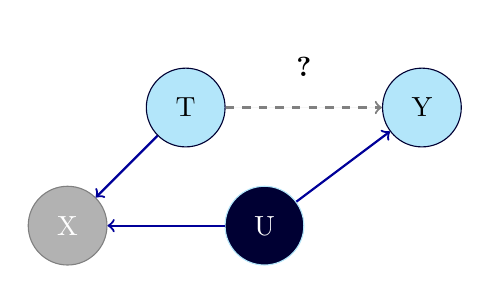
\begin{tikzpicture}[
        darkblue/.style={circle, draw=blue!20!black, fill=cyan!30, text=black, minimum size=1cm},
        blue/.style={circle, draw=cyan!30, fill=blue!20!black, text=white, minimum size=1cm},
        gray/.style={circle, draw=gray, fill=gray!60, text=white, minimum size=1cm},
        lightblue/.style={circle, draw=cyan!50, fill=cyan!15, text=black, minimum size=1cm},
        node distance=2.5cm
    ]
    
    % Left diagram - Confounder
    \node[darkblue, align=center] (T1) at (1.5, 1) {T};
    \node[darkblue, align=center] (Y1) at (4.5, 1) {Y};
    \node[blue] (u) at (2.5, -0.5) {U};
    \node[gray] (X1) at (0, -0.5) {X};
    \draw[->, thick, blue!60!black] (T1) -- (X1);
    \draw[->, thick, blue!60!black] (u) -- (Y1);
    \draw[->, thick, blue!60!black] (u) -- (X1);
    % \draw[->, thick, gray, dashed] (u) -- (X1);
    % \draw[->, thick, blue!60!black] (X1) -- (Y1);
    \draw[->, thick, dashed, gray] (T1) -- node[above, font=\bfseries, text=black] {?} (Y1);
    \end{tikzpicture}
\end{center}
\begin{itemize}
    \item Our previously netral control X \textbf{turns into a bad control}, if there is an unobserved confounder between X and Y
    \begin{itemize}
        \item The initially unbiased T on Y effect becomes biased when including X as a control 
        \item X does not need to have an effect on Y if the relationship is confounded
    \end{itemize}
\end{itemize}
\subsection{Conclusion: any outcomes of T or Y are bad controls}
\begin{itemize}
    \item In almost all cases outcomes of T or Y are bad control variables
    \begin{itemize}
        \item All post-treatment outcomes 
        \item They either hurt precision or bias the effect
    \end{itemize}
    \item Exception: you are interested in direct effect mediation and have no confounders on X-Y
    \begin{itemize}
        \item How likely is it?
    \end{itemize}
    \item Typical recommendation in many textbooks is to include \textbf{only pre-treatment} variables as controls 
    \begin{itemize}
        \item This is often correct, but not always 
    \end{itemize}
\end{itemize}
\newpage
\section{Continuing with treatment effects}
Recall Average Treatment Effect (ATE): 
\begin{itemize}
    \item If requirements are fulfulled, a comparison of average outcomes in treatment and control groups, the so-called difference-in-means, is a consistent estimator of the ATE
\end{itemize}
\subsection{The problem with ATE}
\begin{itemize}
    \item The ATE focuses on the population 
    \item We are averaging over all individuals $i $
    \begin{itemize}
        \item Some individuals might be affected by the treatment and others don't
        \item Some individuals might be more strongly affected by the treatment
    \end{itemize}
    \item There may be heterogeneous treatment effects 
    \item We have already discussed heterogeneous treatment effects when we had ATET $\neq $ ATEU
    \begin{itemize}
        \item Treated and untreated individuals differ in their treatment effects (selection on returns)
        \item It involves some form of selection effects (it does not happen if treatment is independent of potential outcomes; e.g., if treatment is randomized)
    \end{itemize}
    \item However, treatment effects can also be heterogeneous in randomized experiments
\end{itemize}

\subsubsection{Conditional Treatment Effects (CATE)}
\begin{itemize}
    \item The ATE conditioal on membership in a sub-group $M_i = m $
    \begin{itemize}
        \item e.g., for all individuals s.t. $M_{\text{device}} = \text{Apple} $
        \begin{gather*}
            \tau(x) = \mathbb{E}[\tau_i | M_i = m] = \mathbb{E}[Y_i(1) - Y_i(0) | M_i = m]
        \end{gather*}
    \end{itemize}
\end{itemize}
\textbf{Challenges}
\begin{itemize}
    \item Again $\mathbb{E}[\tau_i | M_i = m] $ is not directly observable, so we need to estimate it 
    \begin{itemize}
        \item If assumptions hold, we can do groups-specific ATEs: 
        \begin{gather*}
            \tau(m) = \mathbb{E}[Y_i | T_i = 1, M_i = m] - \mathbb{E}[Y_i | T_i = 0, M_i = m]
        \end{gather*}
    \end{itemize}
    \item Potentialy many ways of creating sub-groups
    \begin{itemize}
        \item We can define a-priori sub-groups and estimate ATE 
        \item We can let the data speak and estimate sub-groups with distinct CATEs
        \begin{itemize}
            \item Causal trees, causal forests, other recent ML-based advancements 
        \end{itemize}
    \end{itemize}
\end{itemize}
\newpage
\subsection{Compliance}
\textbf{Non-compliance}
\begin{itemize}
    \item Potential problem in a randomized experiment --- typically field experiments 
    \item Individuals are assigned to treatment or control, but may not comply with this assignment, e.g., they may receive the opposite of their assignment
    \begin{itemize}
        \item Compliers
        \item Always-takers 
        \item Never-takers 
        \item Defiers
    \end{itemize}
    \item One-sided non-compliance 
    \begin{itemize}
        \item \textbf{Only treatment group} individuals may not comply with the assignment 
        \begin{itemize}
            \item Treatment individuals might receive treatment or not: $D_i(T_i = 1)\in \{0, 1\}  $
            \item Control individuals always receive no treatment: $D_i(T_i = 0) = 0 $
            \item We have \textbf{compliers} and \textbf{never-takers}
        \end{itemize}
        \item Only control group individuals may not comply with the assignment 
        \begin{itemize}
            \item Treatment individuals always receive treatment: $D_i(T_i = 1) = 1$
            \item Control individuals might receive treatment or not: $D_i(T_i = 0)\in \{0, 1\}  $
            \item We have \textbf{compliers} and \textbf{always-takers}
        \end{itemize}
    \end{itemize}
    \item Two-sided non-compliance 
    \begin{itemize}
        \item \textbf{Both treatment and control group} individuals may not comply with the assignment
        \item It's harder to estimate appropriate treatment effects in this situation, but possible as long as there are no defiers; However, we will mostly focus on one-sided non-compliance
    \end{itemize}
\end{itemize}
\subsubsection{Intent to treat (ITT)}
\begin{itemize}
    \item \textbf{Under non-compliance} the intent to treat (ITT) is another treatment effect 
    \begin{itemize}
        \item The treatment effect is estimated based on \textbf{assignment and not actual treatment }
    \end{itemize}
    \item When we have $T_i \in \{0, 1\}$ assigned treatment and $D_i \in \{0, 1\} $ received treatment, then 
    \begin{gather*}
        \tau_{\text{ITT}} = \mathbb{E}[Y_i | T_i = 1] - \mathbb{E}[Y_i | T_i = 0]
    \end{gather*}
    \item Under non-compliance, this is usually different from ATE, because $T_i \neq D_i $, for some $i $
    \item ITT is a valid estimate of the \textbf{effect of the assignment}, but \underline{not} the \textbf{effect of treatment}
    \begin{itemize}
        \item It may give a realistic estimate of the population effect in the real world, where some individuals may not comply, but not an estimate of the focal treatment effect 
    \end{itemize}
\end{itemize}
\newpage
\subsubsection{Local average treatment effect (LATE)}
\begin{itemize}
    \item LATE is another typical treatment effect under non-compliance 
    \begin{itemize}
        \item Local: we focus on compliers; i.e., those that adhere to the assignment 
        \item Assuming randomization of $T $, excludability and non-interference (SUTVA), monotonicity (no defiers), and relevance (i.e., there are compliers)
    \end{itemize}
    \item LATE is also called the complier average causal effect (CACE)
    \begin{itemize}
        \item Average treatment effect (ATE) among the compliers 
    \end{itemize}
    \item LATE only meaningful if we have no defiers 
    \begin{itemize}
        \item Only compliers, always-takers, and never-takers allowed
    \end{itemize}
    LATE = ATET under one-sided non-compliance in the treatment group 
    \begin{itemize}
        \item i.e., compliers and never-takers, but no always-takers 
        \item LATE = ATE if no treatment heterogeneity because ATE = ATET 
    \end{itemize}
    \item LATE is linked to \textbf{instrumental variable methods} as we will see later in the course 
\end{itemize}
\section{What does this have to do with marketing}
\begin{itemize}
    \item Is it worth spending money on (digital) advertising?
    \item Is there an incremental effect on (digital) advertising?
    \begin{itemize}
        \item What would have happened if the advertising was not present?
        \item The difference in the outcome in the absence and presence of the focal advertisement (treatment)
    \end{itemize}
    \item Again: advertising exposure is not random. People are explicitly targeted for advertising where they show interest in the products
    \begin{itemize}
        \item We need a randomized experiment 
    \end{itemize}
    \item Many ad platforms offer tools for ad experiments; i.e., randomized AB tests
\end{itemize}
\subsection{The problem of divergent delivery}
\begin{itemize}
    \item In online ad experiments, tehre is often a difference between assigned to an experimental group and those that are actually exposed to the ad 
    \item Randomization is based on the user-level
    \begin{itemize}
        \item All users who are eligible to see the ad; i.e., fulfill basic requirements of the targeting profile 
    \end{itemize}
    \item But not all users in the treatment group will be exposed to a treatment 
    \item The targeting and real-time auctioning process exposes users to the ads depending on their consumer profile, a prediction of whether they are likely to respond, and competitors' bidding behavious 
    \begin{itemize}
        \item Consequently, the exposed users are not a random sample of eligible users
    \end{itemize}
\end{itemize}
\newpage 
\subsection{Two main types of online ad experiments --- divergent delivery}
\textbf{Single-ad study with holdout/control}
\begin{itemize}
    \item Typical question: is there an incremental effect of the ad on an outcome of interest?
    \item Consumers are randomly divided into a treatment group and a holdout/control group 
    \item Consumers in the treatment group are eligible to see the ad, but not all consumers will see the ad 
    \item Consumers in the holdout/control group will not see the ad 
    \begin{itemize}
        \item One-sided compliance, we are able to calculate LATE or even ATET in some situations 
    \end{itemize}
\end{itemize}
\textbf{Multiple-ad study without holdout}
\begin{itemize}
    \item Typical question: which of the two versions of the ad is better?
    \item Classic AB testing: consumers are randomly assigned to group A or B
    \item Consumers in group A will only see ad A and vice-versa 
    \item Not all consumers will see the ad because of targeting 
    \begin{itemize}
        \item We are not able to make inferences about incremental effects of A over B; i.e., about causal effects 
    \end{itemize}
\end{itemize}
\subsection{Interpretation of AB-test (multiple ad-study) with targeting}
\begin{itemize}
    \item Under divergent delivery, results must be interpreted as the combined effect of ad content and platform's targeting 
    \begin{itemize}
        \item Whether this matters to the experimenter depends on the goal the experiment
    \end{itemize}
    \item You cannot say that ad A is better than ad B (in general or for the specified audience)
    \item You can only say that ad A is better on this platform given the specific targeting algorithm and campaign settings 
    \item Advertisement B might be similar or better thn A 
    \begin{itemize}
        \item On a different platform (with different algos) with different everything
    \end{itemize}
\end{itemize}
\subsection{Conclusions}
\begin{itemize}
    \item Significant selection effects usually lead to overestimating the ad effect 
    \item Observational methods are ususally not able to estimate the ad effect well enough: 
    \begin{itemize}
        \item Even with excessive control variables they overestimate in most studies 
        \item No single observational method is systematically better 
    \end{itemize}
    \item Randomized experiments (AB testing) is the gold standard to avoid selection effects 
\end{itemize}
\newpage 
\subsection{Summary of estimators and interpretation}
\textbf{Assumption}: randomization + SUTVA + monotonicity

\textbf{Full compliance}
\begin{itemize}
    \item ATE = Average treatment effect; ATE = ITT = ATET = LATE 
    \begin{itemize}
        \item e.g., what is the average effect on the entire population
    \end{itemize}
\end{itemize}
\textbf{Non-compliance} (not all individuals comply with treatment assignment; e.g., targeting)
\begin{itemize}
    \item ITT = Intent to treat (compares groups by assignment, and not treatment)
    \begin{itemize}
        \item ITT assesses the treatment's effectiveness for all customers, accounting for non-compliance 
        \item e.g., what is the average effect of an ad, given that some people will not see it 
    \end{itemize}
    \item ATET = average treatment effect on the treated (compare treated against those that would have been treated, if they were not in the control group)
    \begin{itemize}
        \item ATET assesses the treatment's effectiveness only for those that receive treatment
    \end{itemize}
    \item LATE = local average treatment effect (among the compliers); estimate of ATET given assumptions
\end{itemize}
\subsection{Remember: when is LATE = ATET?}
\begin{itemize}
    \item \textbf{One-sided non-compliance}
    \begin{itemize}
        \item When the treatment is only available to the treatment group, the compliers are exactly the same group as the treated population (ATET)
        \item We only have compliers and never-takers, or $D_i(T_i) = 1 $ onlt for $T_i = 1 $
    \end{itemize}
    \item \textbf{Perfect compliance}
    \begin{itemize}
        \item If every individual complies with their assignment
        \item i.e., $p(\text{complier}) = 1 \text{ or } D_i(T_i) = T_i $
    \end{itemize}
    \item \textbf{Homogenous effect}
    \begin{itemize}
        \item If the effect of compliers and non-compliers will be the same 
        \item i.e., there is \textbf{no treatment affect heterogeneity}
        \item In this situation LATE = ATET = ATE 
    \end{itemize}
\end{itemize}
\subsection{Type of treatment effect}
\begin{itemize}
    \item It is important to understand which treatment effects are estimating / are able to estimate in a given situation 
    \item This frames your ability to interpret the effect and to which defree you can generalize 
\end{itemize}
\newpage 
\subsection{Key concepts --- summary}
\begin{itemize}
    \item Individuals usually vary in their strength of the treatment effect 
    \begin{itemize}
        \item Instead of looking only at averages we can also try to explore heterogeneity in the treatment effects $\to $ estimate a CATE 
        \begin{itemize}
            \item e.g., group specific estimates, interaction effects 
        \end{itemize}
    \end{itemize}
    \item Individuals might not always comply with treatment assignment 
    \begin{itemize}
        \item One-sided or two-sided non-compliance
        \item Compliers, always-takers, never-takers, defiers 
        \item Treatment effect estimators: ITT, ATET and LATE 
    \end{itemize}
    \item For measuring (online) advertising effectiveness we need properly designed experiments 
    \begin{itemize}
        \item We need understanding about one-sided non-compliance, etc. 
        \item Even excessive amounts of control variables (e.g., Facebook data) are not able to properly control for all selection effects 
    \end{itemize}
\end{itemize}

\end{document}